\documentclass{oxmathproblems}
\usepackage{graphicx}
\usepackage{listings}
\graphicspath{{imagenes/}} 

\course{HW 4 Heterogeneous Graphs}
\begin{document}
\vspace{-15mm}

We enumerate the graphs based on the total number of edges. By property of \emph{Complementarity}, we only need to enumerate graphs with edge numbers ranging from $0$ to $5$.

\begin{enumerate}
    \item We have 1 graph for 0 edge.
    \item We have 1 graph for 1 edge, shown in Figure \ref{fig:1}.
    \item We have 2 graph for 2 edges, showin in Figure \ref{fig:2}.
    \item We have 4 graphs for 3 edges, showin in Figure \ref{fig:3}.
    \item We have 6 graphs for 4 edges, showin in Figure \ref{fig:4}.
    \item We have 6 graphs for 5 edges, showin in Figure \ref{fig:4}, where the second and third graphs are symmetric, and the fourth and fifth graphs are also symmetric. The first and sixth graphs are symmetric with respect to themselves respectively.
\end{enumerate}

Totally, we have $(1+1+2+4+6)*2 + 6 = 34 $ heterogeneous graphs.

\begin{figure}[hb]
  \begin{center}
  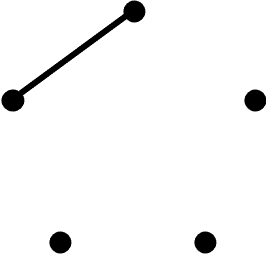
\includegraphics[height=2cm]{img/4-1.png}
  \caption{Heterogeneous Graphs with 1 edge}
  \label{fig:1}
  \end{center}
\end{figure}


\begin{figure}[hb]
    \begin{center}
    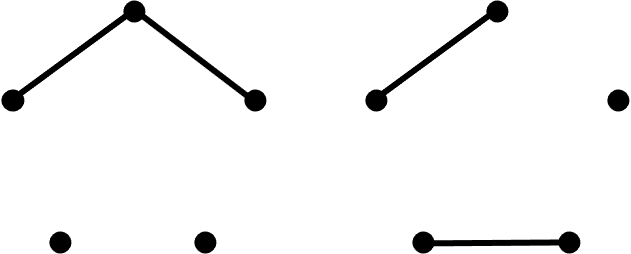
\includegraphics[height=2cm]{img/4-2.png}
    \caption{Heterogeneous Graphs with 2 edges}
    \label{fig:2}
    \end{center}
\end{figure}


\begin{figure}[hb]
    \begin{center}
    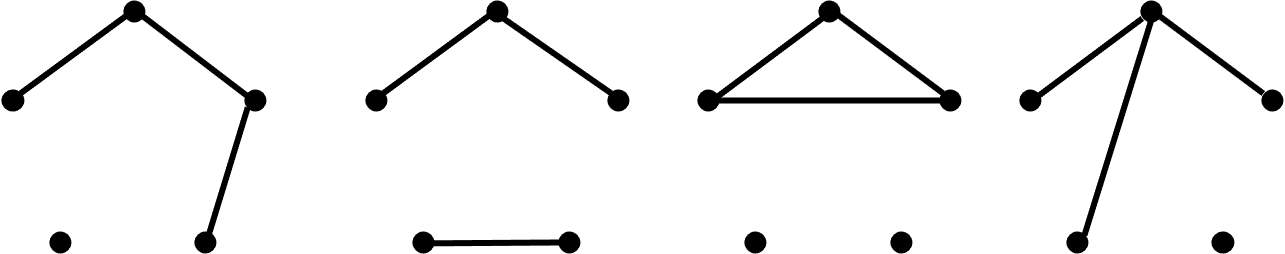
\includegraphics[height=2cm]{img/4-3.png}
    \caption{Heterogeneous Graphs with 3 edges}
    \label{fig:3}
    \end{center}
\end{figure}


\begin{figure}[hb]
    \begin{center}
    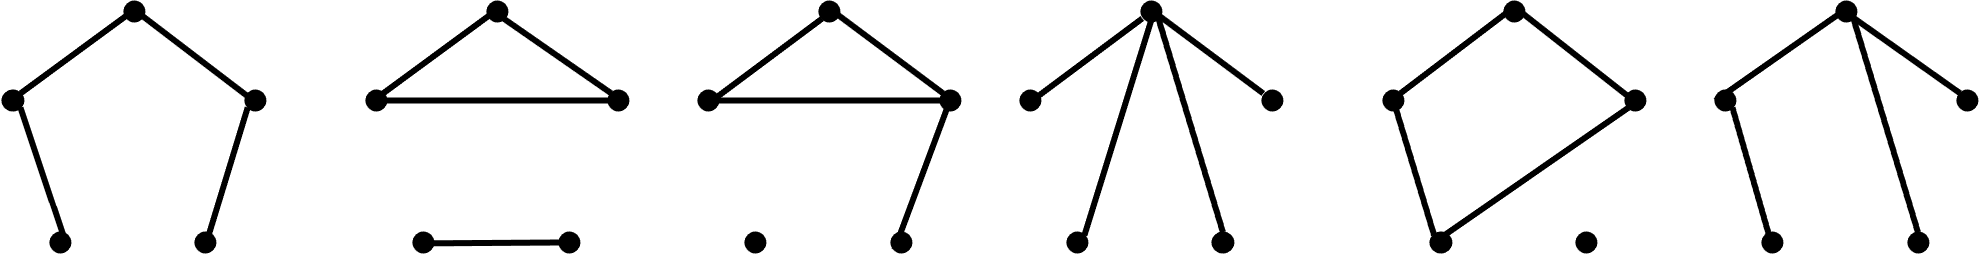
\includegraphics[height=2cm]{img/4-4.png}
    \caption{Heterogeneous Graphs with 4 edges}
    \label{fig:4}
    \end{center}
\end{figure}


\begin{figure}[hb]
    \begin{center}
    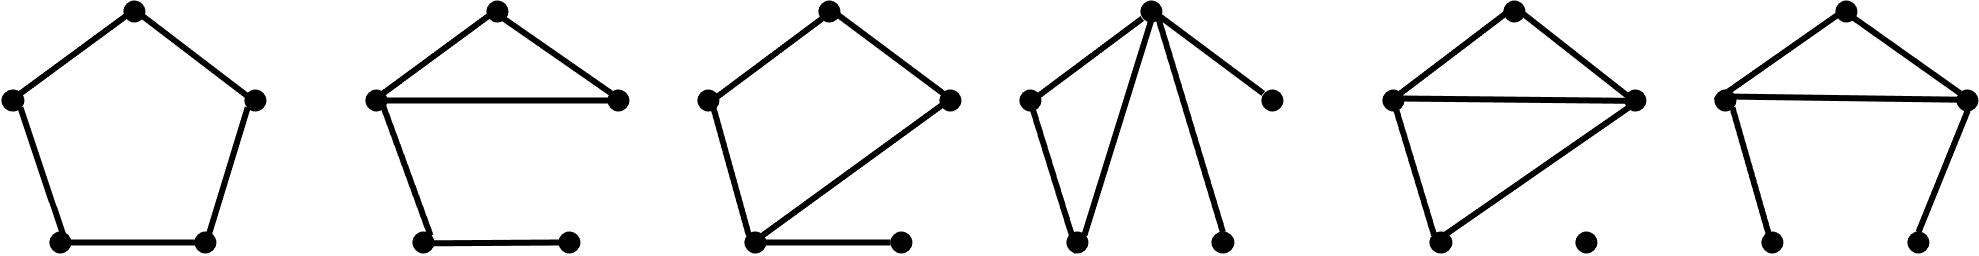
\includegraphics[height=2cm]{img/4-5.png}
    \caption{Heterogeneous Graphs with 5 edges}
    \label{fig:5}
    \end{center}
\end{figure}


\end{document}
